\documentclass[a4paper,11pt]{ctexart}
\usepackage{amssymb}
\usepackage{amsmath}

\usepackage{graphicx}
\usepackage{geometry}
\geometry{top=2.5cm, bottom=1.8cm, left=2cm, right=2.5cm}

%================ 行距 ================
\usepackage{setspace}
\setstretch{1.3}

\usepackage{calc}
\setlength{\lineskip}{\baselineskip-\ccwd}
\setlength{\lineskiplimit}{2.5pt}

\usepackage{enumitem}
\usepackage{listings}
\lstset{
    basicstyle          =   \sffamily,          % 基本代码风格
    keywordstyle        =   \bfseries,          % 关键字风格
    commentstyle        =   \rmfamily\itshape,  % 注释的风格，斜体
    stringstyle         =   \ttfamily,  % 字符串风格
    flexiblecolumns,                % 别问为什么，加上这个
    numbers             =   left,   % 行号的位置在左边
    showspaces          =   false,  % 是否显示空格，显示了有点乱，所以不现实了
    numberstyle         =   \zihao{-5}\ttfamily,    % 行号的样式，小五号，tt等宽字体
    showstringspaces    =   false,
    captionpos          =   t,      % 这段代码的名字所呈现的位置，t指的是top上面
    frame               =   lrtb,   % 显示边框
}

\renewcommand{\d}{\mathop{}\!\mathrm{d}}
\everymath{\displaystyle}


\begin{document}

\title{微分方程数值解作业1}
\author{庞逸天 523070910095}
\maketitle

\section{习题 1}

生成图片的matlab代码为：
\begin{lstlisting}[language=Matlab]
    [x,y] = meshgrid(-5:1/10:5)
    z = x.^2 + y.^2
    surf(x,y,z), shading interp; colorbar
\end{lstlisting}

对应得到的图像为：
\begin{figure}[htbp]
    \centering
    
\includegraphics[width=0.8\textwidth]{1.pdf}
\end{figure}

\section{习题 2}

生成图片的matlab代码为：
\begin{lstlisting}[language=Matlab]
    r = 1.0;
    d = 0.5;
    a = 0.1;
    b = 0.02;

    t_final = 1000;
    x0 = [100,2.0];

    voterra = @(t,x)[x(1) * (r - a * x(2));
        x(2)*(-d + b * x(1))];

    [t,x] = ode45(voterra,[0,t_final],x0);
        plot(x(:,1),x(:,2))
\end{lstlisting}

所得到的轨线图为：
\begin{figure}[htbp]
    \centering
    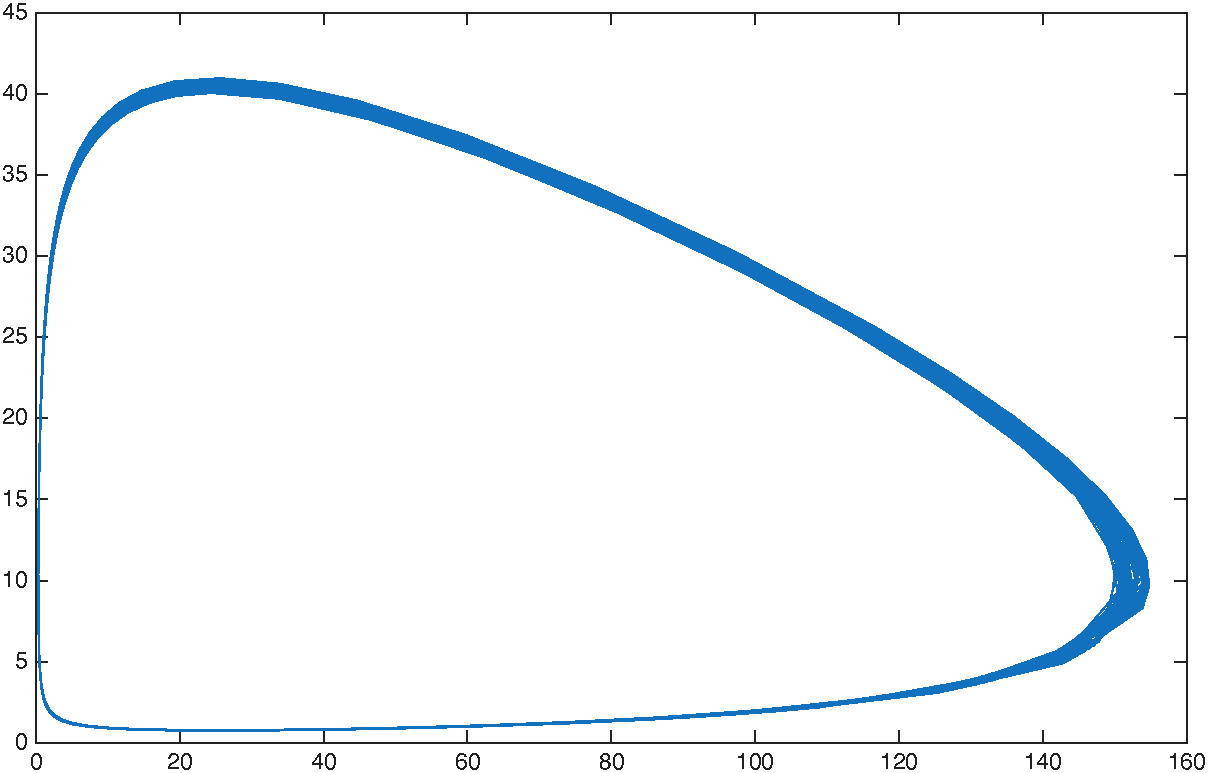
\includegraphics[width=0.8\textwidth]{2.pdf}
\end{figure}

\section{习题 3}

首先由Fourier热传导定律可知$\d Q=-k\partial_n u\d S\d t$，其中$u(x)$为$x$处的温度，$S$为横截面积，$f(x)$为热源密度，$k(x)$为热传导系数.\par
在单位时间内，考虑微元$[x,x+\Delta x]$的热量变化.\par
产热为$\Delta Q=f(x)\Delta x S$，流出的热量为$\Delta Q'=-ku'(x+\Delta x)S+ku'(x)S$.\par
杆子侧面绝热，因此由能量守恒定律，$\Delta Q=\Delta Q'$，即$f(x)\Delta x S=-(ku')(x+\Delta x)S+(ku')(x)S$.\par
$\Rightarrow \frac{(ku')(x+\Delta x)-(ku')(x)}{\Delta x}=f(x)$.\par
下面令$\Delta x\to 0$，由于$k(x)$是一个分段函数，因此需要分类讨论.\par
\begin{enumerate}[label=(\arabic*)]
    \item 当$x\in \left(0,\frac{1}{2}\right)$时，$k(x)=k_1$，因此$-(ku')'(x)=f(x)$，即$-k_1u''(x)=f(x)$.
    \item 当$x\in \left(\frac{1}{2},1\right)$时，$k(x)=k_2$，因此$-(ku')'(x)=f(x)$，即$-k_2u''(x)=f(x)$.
    \item 当$x=\frac{1}{2}$时，温度必须是连续的，因此$\lim_{x\to \frac{1}{2}^-}{u(x)}=\lim_{x\to\frac{1}{2}^+}{u(x)}$.\par
    除此之外，由于热源遍布整个金属杆，故热流密度也应当是连续的，因此$\lim_{x\to \frac{1}{2}^-}{ku'(x)}=\lim_{x\to\frac{1}{2}^+}{ku'(x)}$，即$k_1\lim_{x\to \frac{1}{2}^-}{u'(x)}=k_2\lim_{x\to\frac{1}{2}^+}{u'(x)}$
\end{enumerate}
综上，最终的数学模型由分段的微分方程，中间值的正则性条件以及边界条件组成，具体为：
\[\begin{cases}
-k_1u''(x)=f(x), x\in \left(0,\frac{1}{2}\right)\\[10pt]
-k_2u''(x)=f(x), x\in \left(\frac{1}{2},1\right)\\[10pt]
\lim_{x\to \frac{1}{2}^-}{u(x)}=\lim_{x\to\frac{1}{2}^+}{u(x)}\\
k_1\lim_{x\to \frac{1}{2}^-}{u'(x)}=k_2\lim_{x\to\frac{1}{2}^+}{u'(x)}\\
u(0)=u(1)=0
\end{cases}\]

\section{习题 4}

设$v,\lambda$是$A$的特征值和特征向量，则$Av=\lambda v$.设$v=(v_1,v_2,\cdots,v_N)$.\par
则$Av=\begin{bmatrix}
    0 & 1 & &\\
    1 & \ddots & \ddots & \\
    & \ddots & \ddots & 1\\
    & & 1 & 0
\end{bmatrix}\begin{bmatrix}
    v_1\\
    v_2\\
    \vdots\\
    v_N
\end{bmatrix}=\begin{bmatrix}
    v_2 \\
    v_1+v_3\\
    \vdots\\
    v_{N-1}
\end{bmatrix}$，因此$\begin{cases}
v_2=\lambda v_1\\
v_1+v_3=\lambda v_2\\
\vdots\\
v_{N-1}=\lambda v_N
\end{cases}$.\par
令$v_0=v_{N+1}=0$，则可将上述方程组改写为$\begin{cases}
    v_2=\lambda v_1 + v_0 \\
    v_3=\lambda v_2 + v_1\\
    \vdots\\
    v_{N+1}=\lambda v_{N} + v_{N-1}
\end{cases}$.\par
即$v_i$满足二阶线性递推关系$v_i=\lambda v_{i-1}+v_{i-2},v_0=v_{N+1}=0,i\geq 2$.\par
上述递推关系的特征方程为$r^2-\lambda r-1=0$，解得$r=\frac{\lambda\pm\sqrt{\lambda^2-4}}{2}$.\par
令$\lambda=2\cos\theta$，则$r=\frac{2\cos\theta\pm\sqrt{4\cos^2\theta-4}}{2}=\cos\theta\pm i\sin\theta=e^{\pm i\theta}$.\par
因此$v_i$的通解为$v_k=C_1e^{i\theta k}+C_2e^{-i\theta k}$.\par
由$v_0=0$可知$v_0=C_1+C_2=0$，即$C_2=-C_1$.\par
将其带入$v_k$中，得$v_k=C_1 e^{i\theta k}-C_1 e^{-i\theta k}=2C_1\sin(\theta k)$.\par
由$v_{N+1}=0$可知$2C_1\sin(\theta(N+1))=0$.\par
由于特征向量非零，故$C_1\neq 0$，只有$\sin(\theta(N+1))=0$，从而$(N+1)\theta=m\pi$.\par
故$\theta=\frac{m\pi}{N+1},1\leq m\leq N$.\par
将$\theta$带入$v_k$表达式中，即得到$v_k=C\sin\left(\frac{km}{N+1}\pi\right)$.\par
综上所述，上述矩阵的特征值为$\lambda_m=2\cos\frac{m}{N+1}\pi,1\leq m\leq N$，对应的特征向量为$v_m=\left(\sin\frac{m}{N+1}\pi,\sin\frac{2m}{N+1}\pi,\cdots,\sin\frac{Nm}{N+1}\pi\right)$






\end{document}
